% The contents of this file is 
% Copyright (c) 2009-  Charles R. Severance, All Righs Reserved

\chapter{웹서비스 사용하기}
프로그램을 사용하여 HTTP상에서 문서를 가져오고 파싱하는 것이 쉽게 되면, 다른 프로그램에서 
활용되도록 특별히 설계된 문서(즉, 브라우져에서 HTML로 보여지지 않는 것)를 생성하는 방법을 개발하는 것은 오래 걸리지 않는다.

웹상에서 데이터를 교환할 때 두 가지 일반적인 형식이 있다.
XML(``eXtensible Markup Language'')은 오랜 기간 사용되어져 왔고 문서형식 데이터를 교환하는데 적절하다.
딕셔너리, 리스트 혹은 다른 내부 정보를 프로그램으로 서로 교환할 때, JSON(JavaScript Object Notation, \url{www.json.org})을 사용한다. 두 가지 형식에 대해서 살펴볼 것이다.

\section{XML(eXtensible Markup Language)}
XML은 HTML과 매우 유사하지만, XML은 좀더 HTML보다 구조화되었다.
여기 XML 문서 샘플이 있다.

\beforeverb
\begin{verbatim}
<person>
  <name>Chuck</name>
  <phone type="intl">
     +1 734 303 4456
   </phone>
   <email hide="yes"/>
</person>
\end{verbatim}
\afterverb
%

종종 XML문서를 나무 구조로 생각하는 것이 도움이 된다. 최상단 {\tt person} 태그가 있고
{\tt phone} 같은 다른 태그는 부모 노드의 \emph{자식(children)} 노드로 그려진다.

\beforefig
\centerline{\includegraphics[height=1.50in]{figs2/xml-tree.eps}}
\afterfig

\section{XML 파싱}

\index{ElementTree}
\index{ElementTree!fromstring}
\index{ElementTree!find}

다음은 XML을 파싱하고 XML에서 데이터 요소를 추출하는 간단한 응용프로그램이다.

\beforeverb
\begin{verbatim}
import xml.etree.ElementTree as ET

data = '''
<person>
  <name>Chuck</name>
  <phone type="intl">
     +1 734 303 4456
   </phone>
   <email hide="yes"/>
</person>'''

tree = ET.fromstring(data)
print 'Name:',tree.find('name').text
print 'Attr:',tree.find('email').get('hide')
\end{verbatim}
\afterverb
%

{\tt fromstring}을 호출하여 XML 문자열 표현식을 XML 노드의 '나무(tree)'로 변환한다.
XML이 나무구조로 되어 있을 때, XML에서 데이터의 일부분을 추출하기 위해서 호출할 일련의 메쏘드가 있다.

{\tt find} 함수는 XML 나무를 훑어서 특정 태그와 매칭되는 {\bf 노드(node)}를 검색한다. 
각 노드는 텍스트, 속성(즉, hide 같은), 그리고 ''자식(child)'' 노드로 구성된다. 각 노드는 노드 나무의 최상단이 될 수 있다.

\beforeverb
\begin{verbatim}
Name: Chuck
Attr: yes
\end{verbatim}
\afterverb
%

{\tt ElementTree}같은 XML 파서를 사용하는 것은 잇점이 있는데 상기 예제의 XML은 매우 간단하지만,
적합한 XML에 대한 많은 규칙이 있고, {\tt ElementTree}를 사용해서 XML 구문 규칙에 얽매이지 않고 XML에서
데이터를 추출할 수 있다.

\section{노드 반복하기}

\index{ElementTree!findall}
\index{ElementTree!get}

종종 XML은 다중 노드를 가지고 있어서 모든 노드를 처리하기 위해서 루프를 작성할 필요가 있다.
다음 프로그램에서 모든 {\tt user} 노드를 루프로 반복한다.

\beforeverb
\begin{verbatim}
import xml.etree.ElementTree as ET

input = '''
<stuff>
    <users>
        <user x="2">
            <id>001</id>
            <name>Chuck</name>
        </user>
        <user x="7">
            <id>009</id>
            <name>Brent</name>
        </user>
    </users>
</stuff>'''

stuff = ET.fromstring(input)
lst = stuff.findall('users/user')
print 'User count:', len(lst)

for item in lst:
    print 'Name', item.find('name').text
    print 'Id', item.find('id').text
    print 'Attribute', item.get('x')
\end{verbatim}
\afterverb
%

{\tt findall} 메쏘드는 XML 나무의 {\tt user} 구조를 표현하는 파이썬 리스트의 하위 나무를 가져온다.
그리고 나서, {\tt for} 루프를 작성해서 {\tt user} 노드의 각 값을 확인하고 {\tt name}, {\tt id} 텍스트 요소와 
{\tt user} 노드에서 {\tt x} 속성을 출력한다.

\beforeverb
\begin{verbatim}
User count: 2
Name Chuck
Id 001
Attribute 2
Name Brent
Id 009
Attribute 7
\end{verbatim}
\afterverb
%

\section{JSON(JavaScript Object Notation)}
\index{JSON}
\index{JavaScript Object Notation}

JSON 형식은 자바스크립트 언어에서 사용되는 개체와 배열 형식에서 영감을 얻었다.
하지만 파이썬이 자바스크립트 이전에 개발되어서 딕셔너리와 리스트의 파이썬 구문이 JSON 구문에 영향을 주었다.
그래서 JSON 포맷이 거의 파이썬의 리스트와 딕셔너리의 조합과 일치한다. 

상기 간단한 XML에 대략 상응하는 JSON으로 작성한 것이 다음에 있다.

\beforeverb
\begin{verbatim}
{
  "name" : "Chuck",
  "phone" : {
    "type" : "intl",
    "number" : "+1 734 303 4456"
   },
   "email" : {
     "hide" : "yes"
   }
}
\end{verbatim}
\afterverb
%

몇가지 차이점에 주목하세요. 첫째로 XML에서는 ''phone'' 태그에 ''intl''같은 속성을 추가할 수 있다.
JSON에서는 단지 키-밸류 페어(key-value pair)다. 또한 XML ''person'' 태그는 사라지고 중괄호 세트로 대체되었다.

일반적으로 JSON 구조가 XML보다 간단하다. 왜냐하면, JSON이 XML보다 적은 역량을 보유하기 때문이다.
하지만 JSON이 딕셔너리와 리스트의 조합에 {\em 직접} 매핑된다는 장점이 있다.
그리고, 거의 모든 프로그래밍 언어가 파이썬 딕셔너러와 리스트에 상응하는 것을 가지고 있어서,
JSON이 두 협업 프로그램이 데이터를 교환하는데 매우 자연스러운 형식이 된다.

XML에 비해서 상대적으로 단순함으로써, JSON은 응용프로그램 간의 거의 모든 데이터를 교환하는데 있어
빠르게 선택되고 있다. 

\section{JSON 파싱하기}
딕셔너리(개체)와 리스트를 중첩함으로써 JSON을 생성한다. 이번 예제에서,
각 user가 딕셔너리로 키-밸류 페어(key-value pair)인 user 리스트를 표현한다. 그래서 리스트 딕셔너리가 있다.

다음 프로그램에서 내장된 {\bf json} 라이브러리를 사용하여 JSON을 파싱하여 데이터를 읽어온다.
이것을 XML과 상응하는 데이터, 코드와 비교해 보세요. JSON은 조금 덜 자세해서 사전에 미리 리스트를 가져올 것이고, user 리스트가 있고 각 user는 키-밸류 페어 집합임을 알 수 있다. JSON은 좀더 간략(장점)하고 하지만 
좀더 덜 서술적(단점)이다. 

\beforeverb
\begin{verbatim}
import json

input = '''
[
  { "id" : "001",
    "x" : "2",
    "name" : "Chuck"
  } ,
  { "id" : "009",
    "x" : "7",
    "name" : "Chuck"
  } 
]'''

info = json.loads(input)
print 'User count:', len(info)

for item in info:
    print 'Name', item['name']
    print 'Id', item['id']
    print 'Attribute', item['x']
\end{verbatim}
\afterverb
%

JSON과 XML에서 데이터를 추출하는 코드를 비교하면, 
{\bf json.loads()} 에서 파이썬 리스트를 얻고,
{\bf for} 루프로 훑고, 리스트 내부의 각 항목은 파이썬 딕셔너리로
각 user의 다양한 정보를 추출하기 위해서 파이썬 인덱스 연산자를 사용한다. 
JSON을 파싱하면, 네이티브 파이썬 개체와 구조가 생성된다.
반환된 데이터가 단순히 네이티브 파이썬 구조체이기 때문에, 파싱된 JSON을 활용하는데
JSON 라이브러리를 사용할 필요는 없다. 
 
프로그램 출력은 정확하게 상기 XML 버젼과 동일한다.

\beforeverb
\begin{verbatim}
User count: 2
Name Chuck
Id 001
Attribute 2
Name Brent
Id 009
Attribute 7
\end{verbatim}
\afterverb
%

일반적으로 웹서비스에 대해서 XML에서 JSON으로 가는 산업 경향이 뚜렷하다.
JSON이 좀더 간단하고 이미 프로그래밍 언어에서 갖고 있는 네이티브 자료 구조와 직접적으로 매핑되기 때문에
파싱하고 데이터 추출하는 코드는 JSON을 사용할 때 좀더 간단하고 직접적이다.
하지만 XML이 JSON보다 좀더 자기 서술적이고 XML이 강점을 가지는 몇몇 어플리케이션이 있다.
예를 들어, 대부분의 워드 프로세서는 JSON보다는 XML을 사용하여 내부적으로 문서를 저장한다. 

\section{API(Application Program Interfaces, 응용 프로그램 인터페이스)}

이제 HTTP를 사용하여 응용프로그램간에 데이터를 교환하고 XML과 JSON을 사용하여 응용프로그램간에도
복잡한 데이터를 주고 받을 수 있는 방법을 습득했다.

다음 단계는 이들 기법을 사용하여 응용프로그램 간에 ''계약(contract)''을 정의하고 문서화하는 것이다.
응용프로그램-대-응용프로그램 계약의 일반적 명칭은 APIs, {\bf 응용 프로그램 인터페이스(Application Program 
Interfaces)}이다. API를 사용할 때, 일반적으로 하나의 프로그램은 다른 응용 프로그램에서 사용되도록
가능한 서비스 집합을 생성하고 프로그램에서 제공하는 서비스에 접근하도록 API (즉, ''규칙'')를 게시한다.  

프로그램의 기능이 다른 프로그램에서 제공되는 서비스에 접근도 포함되도록 프로그램을 개발 할 때,
이러한 개발 접근법을 SOA, {\bf Service-Oriented Architecture(서비스 지향 아키텍처)}라고 부른다.
SOA가 아닌 접근법은 응용 프로그램이 하니의 독립 응용 프로그램으로 구현에 필요한 모든 코드를 담고 있다.

웹을 사용할 때 SOA의 많은 사례를 찾아 볼 수 있다. 하나의 웹사이트를 방문하여 비행기표, 호텔, 자동차를 단일
사이트에서 예약한다. 호텔관련 데이터는 물론 항공사 컴퓨터에 저장되어 있지 않다.
대신에 항공사 컴퓨터는 호텔 컴퓨터와 계약을 맺어 호텔 데이터를 가져와서 사용자에게 보여준다.
사용자가 항공사 사이트를 통해서 호텔 예약을 동의할 경우, 항공사 사이트는 실제 예약을 하기 위해서
호텔 시스템의 또다른 웹서비스를 사용한다.
전체 트랜젝션에 대해서 카드 결재를 할 때, 여전히 다른 컴퓨터가 프로세스에 물려있다.

\beforefig
\centerline{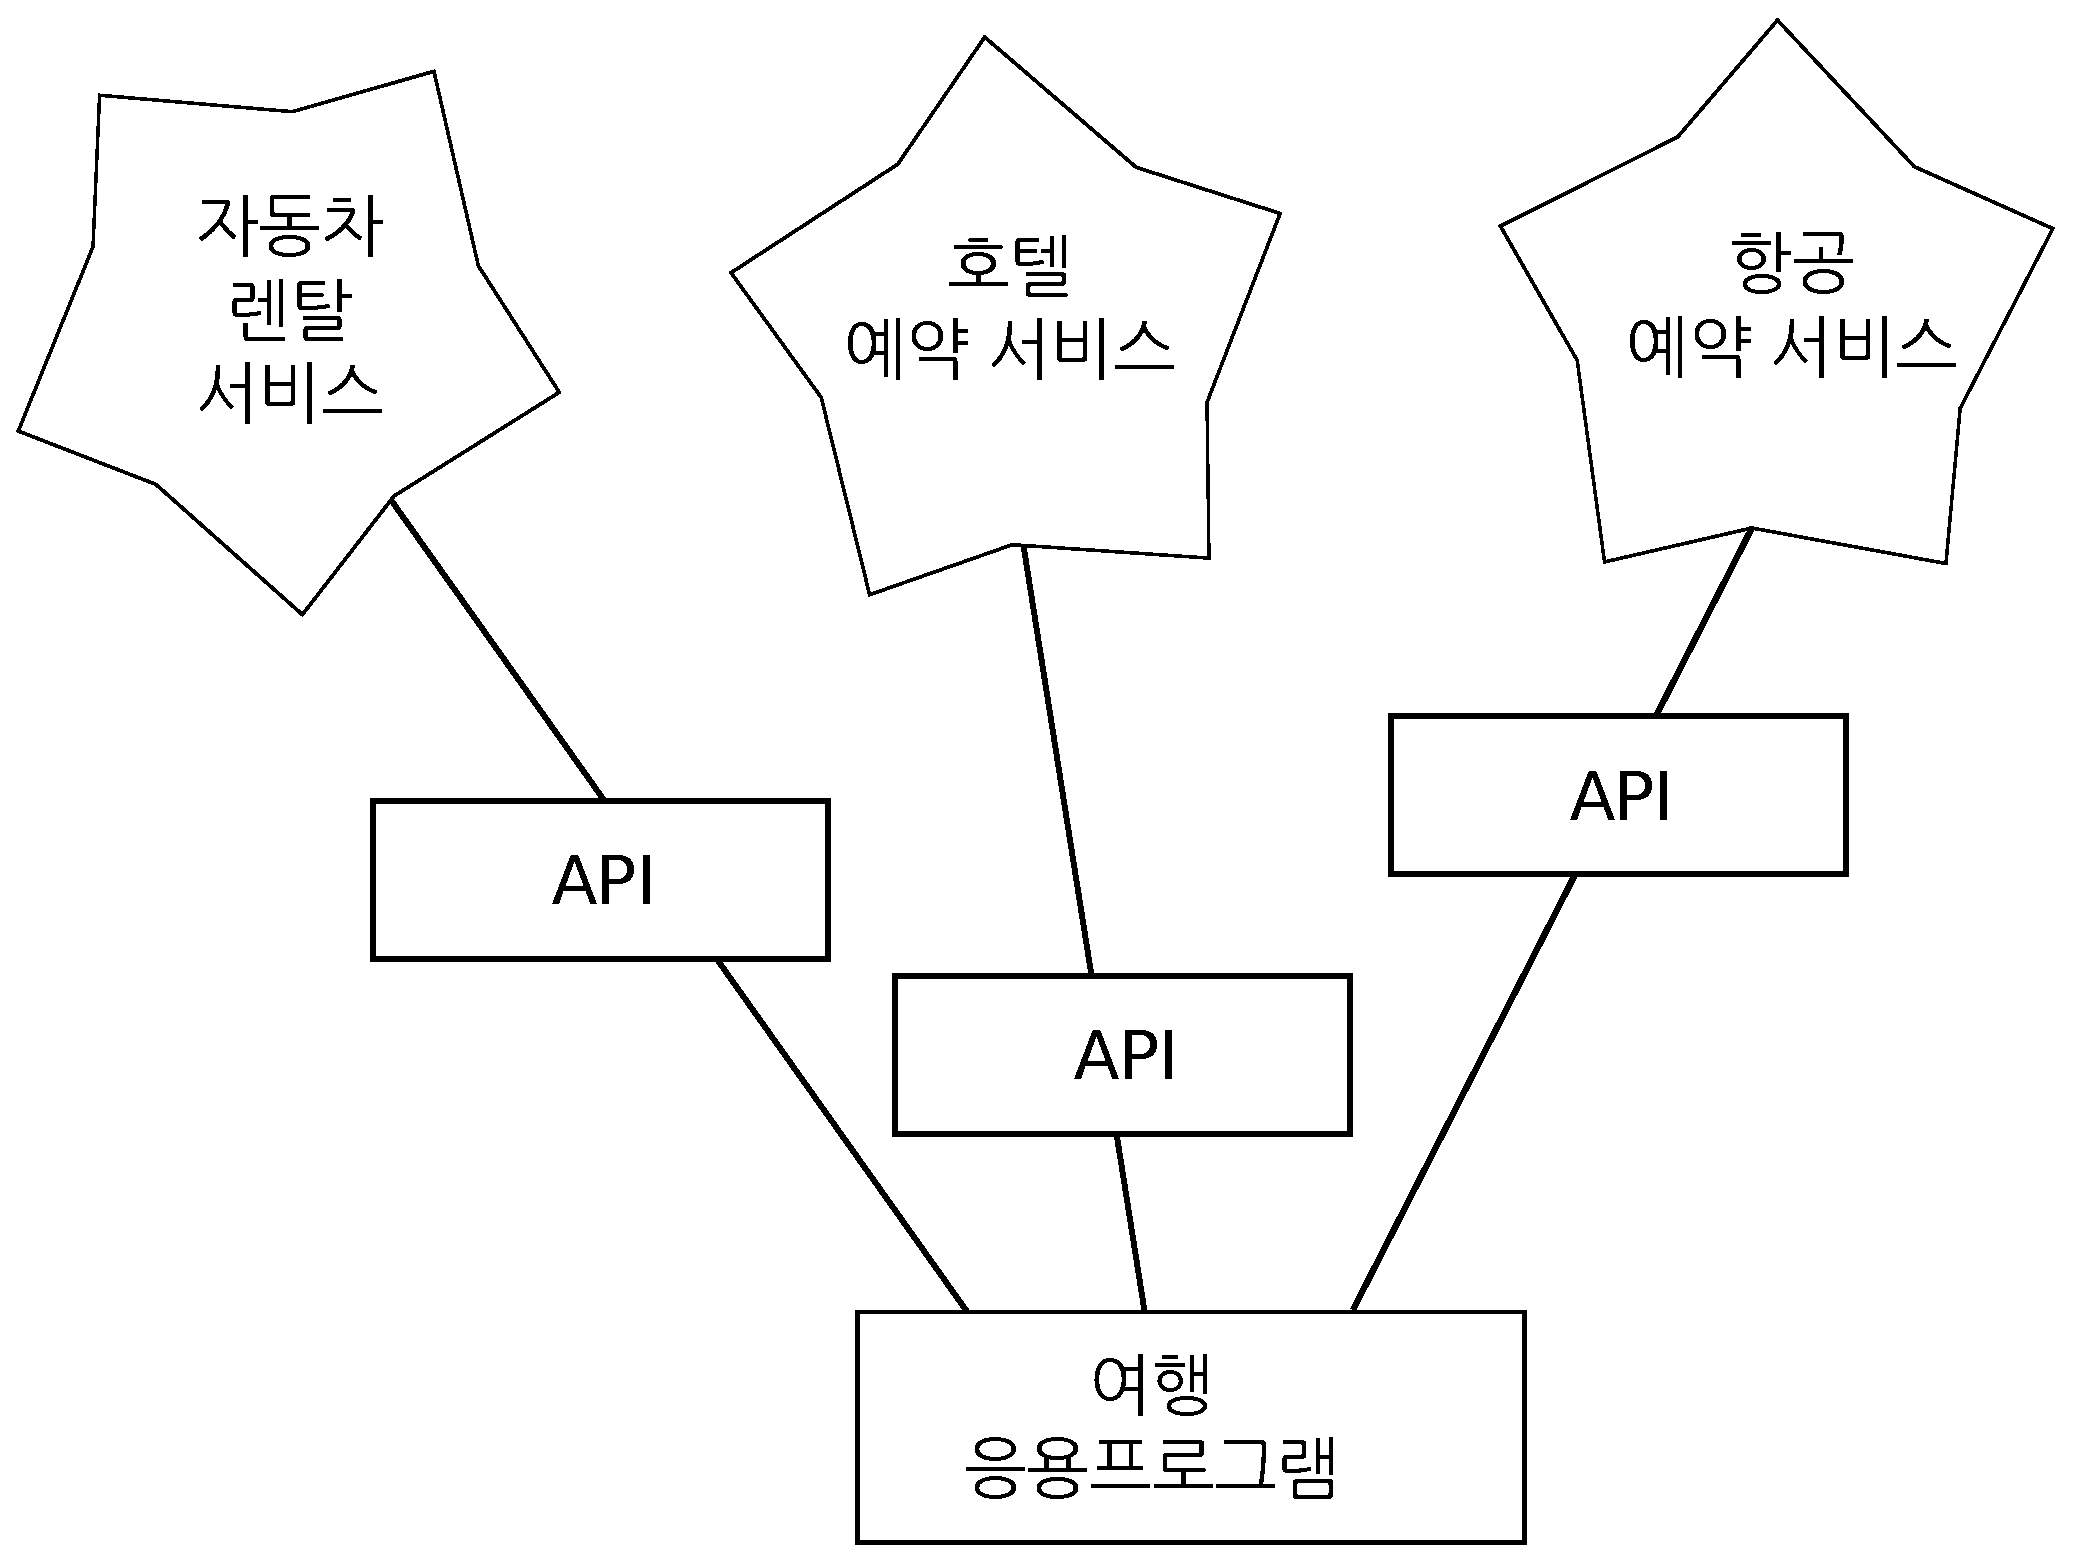
\includegraphics[height=2.50in]{figs2/soa.eps}}
\afterfig

서비스 지향 아키텍쳐는 많은 장점을 지니고 있다. (1) 항상 단 하나의 데이터만 유지관리한다. 
능력 이상으로 예약을 원치않는 호텔  같은 경우에 특히나 중요하다. (2) 데이터 소유자가 
데이터의 사용에 대한 규칙을 정한다. 이러한 장점으로, SOA 시스템은 좋은 성능과 사용자 요구를 만족하기 위해서
주의깊이 설계되어야 한다. 

응응프로그램이 웹상에서 가능한 API 형식의 서비스 집합을 만들 때, {\bf 웹서비스(web services)}라고 부른다.

\section{구글 지오코딩 웹서비스(Google Geocoding Web Service)}
\index{Google}
\index{geocoding}
\index{web service}

구글은 자체적으로 구축한 대용량 지리 정보 데이터베이스를 이용할 수 있게 해주는 훌륭한 웹서비스가 있다.
``Ann Arbor, MI'' 같은 지리적 검색 문자열을 지오코딩 API에 넣으면, 
검색 문자열을 찾아서 지도상에 근처의 주요 지형지물과 함께 최선의 예측치를 보여준다. 

지오코딩 서비스는 무료지만 사용량은 제한되어 있어서, 상업적 응용프로그램에 API를 제한없이 사용할 수는 없다.
하지만, 최종 사용자가 자유형식 입력 박스에 위치정보를 입력하는 설문 데이터가 있다면,
API를 사용하여 데이터를 깔끔하게 정리할 수는데 사용할 수 있다.

{\em When you are using a free API like Google's geocoding API, you need
to be respectful in your use of these resources.  If too many people abuse the
service, Google might drop or significantly curtail its free service.}
\index{rate limiting}

서비스에 대한 온라인 문서를 정독할 수 있지만, 무척 간단해서 브라우저에 다음 URL을 입력함으로써 테스트까지 할 수 있다.

\url{http://maps.googleapis.com/maps/api/geocode/json?sensor=false &address=Ann+Arbor%2C+MI}

URL만 벗겨내고 웹프라우저에 붙여넣기 전에 URL에서 모든 공백이 제거되었는지 확인하세요.

다음은 사용자가 검색 문자열을 입력하고 구글 지오코딩 API를 호출하여 반환된 JSON에서 정보를 추출하는 
간단한 응용프로그램이다.

\beforeverb
\begin{verbatim}
import urllib
import json

serviceurl = 'http://maps.googleapis.com/maps/api/geocode/json?'

while True:
    address = raw_input('Enter location: ')
    if len(address) < 1 : break

    url = serviceurl + urllib.urlencode({'sensor':'false', 
          'address': address})
    print 'Retrieving', url
    uh = urllib.urlopen(url)
    data = uh.read()
    print 'Retrieved',len(data),'characters'

    try: js = json.loads(str(data))
    except: js = None
    if 'status' not in js or js['status'] != 'OK':
        print '==== Failure To Retrieve ===='
        print data
        continue

    print json.dumps(js, indent=4)

    lat = js["results"][0]["geometry"]["location"]["lat"]
    lng = js["results"][0]["geometry"]["location"]["lng"]
    print 'lat',lat,'lng',lng
    location = js['results'][0]['formatted_address']
    print location
\end{verbatim}
\afterverb
%

프로그램은 검색 문자열을 받아서 적절하게 인코딩된 매개 변수로 검색문자열을 가진 URL을 만든다.
그리고 나서 {\bf urllib}을 사용하여 구글 지오코딩 API에서 텍스트를 가져온다.
고정된 웹페이지와 달리, 반환되는 데이터는 전송하는 매개변수와 구글 서비스에 저장된 지리정보 데이터에
의존하게 된다.

JSON 데이터를 가져오면, {\bf json} 라이브러리로 파싱하고 전송받은 데이터가 올바른지 확인하는 몇가지 절차를 거친 후에 찾고자 하는 정보를 추출한다.

프로그램의 출력은 다음과 같다. (몇몇 JSON 출력은 의도적으로 삭제했다.)

\beforeverb
\begin{verbatim}
$ python geojson.py
Enter location: Ann Arbor, MI
Retrieving http://maps.googleapis.com/maps/api/
  geocode/json?sensor=false&address=Ann+Arbor%2C+MI
Retrieved 1669 characters
{
    "status": "OK", 
    "results": [
        {
            "geometry": {
                "location_type": "APPROXIMATE", 
                "location": {
                    "lat": 42.2808256, 
                    "lng": -83.7430378
                }
            }, 
            "address_components": [
                {
                    "long_name": "Ann Arbor", 
                    "types": [
                        "locality", 
                        "political"
                    ], 
                    "short_name": "Ann Arbor"
                } 
            ], 
            "formatted_address": "Ann Arbor, MI, USA", 
            "types": [
                "locality", 
                "political"
            ]
        }
    ]
}
lat 42.2808256 lng -83.7430378
Ann Arbor, MI, USA
Enter location:
\end{verbatim}
\afterverb
%

다양한 구글 지오코딩 API의 XML과 JSON을 좀더 살펴보기 위해서 \url{www.py4inf.com/code/geojson.py},
\url{www.py4inf.com/code/geoxml.py}을 다운로드 받아 보기 바랍니다.

\section{보안과 API 사용}
\index{OAuth}
\index{API!key}

상용업체의 API를 사용하기 위해서 일종의 ''API키(API key)''가 필요한 것이 일반적이다.
서비스 제공자 입장에서는 누가 서비스를 사용하고 있으며 각 사용자가 얼마나 사용하는지를 알고자 한다.
아마도 서비스에 대한 무료와 유료 사용자에 대한 구분이 있거나 특정 기간 동안 한 개인이 사용할 수 있는
요청수에 대한 제한을 두는 정책이 있다. 

때때로 API키를 가지게 되면, POST 데이터의 일부로서 포함하거나 API를 호출할 때
URL의 매개변수로서 단순하게 키를 포함시킨다.

또 다른 경우는 업체가 서비스 요청에 대한 보증을 강화해서 공유키와 비밀번호를 암호화된 메시지 형식으로
보내도록 요구한다. 인터넷을 통해서 서비스 요청을 암호화하는 일반적인 기술을 {\bf OAuth}라고 한다.
\url{http://www.oauth.net} 사이트에서 OAuth 프로토콜에 대해 더 많은 정보를 만날 수 있다. 

트위터 API가 점차적으로 가치있게 됨에 따라 트위터가 공개된 API에서 매번 API 호출시에 OAuth 인증을 사용하는
API로 바뀌었다. 다행스럽게도 편리한 많은 OAuth 라이브러리가 많이 있다. 

그래서 명세서를 읽고 맨바닥에서부터 OAuth 구현을 필할 수 있다. 이용가능한 라이브러리에는 
다양한 복잡성과 풍부성이 있다. OAuth 웹사이트에서 다양한 OAuth 라이브러리 정보를 확인할 수 있다. 

다음 샘플 프로그램으로 \url{www.py4inf.com/code} 사이트에서 {\bf twurl.py}, {\bf hidden.py}, 
{\bf oauth.py}, {\bf twitter1.py} 파일을 다운로드 받아서 컴퓨터에 한 폴더에 저장한다.

프로그램을 사용하기 위해서 트위터 계정이 필요하고, 응용프로그램으로 파이썬 코드를 인증하고,
키, 암호, 토큰과 토큰 암호를 설정해야 한다. 
{\bf hidden.py} 파일을 편집하여 4개 문자열을 파일에 적절한 변수에 저장한다.

\beforeverb
\begin{verbatim}
    def auth() :
        return { "consumer_key" : "h7L...GNg",
            "consumer_secret" : "dNK...7Q",
            "token_key" : "101...GI",
            "token_secret" : "H0yM...Bo" }
\end{verbatim}
\afterverb
%

트위터 웹서비스는 다음 URL을 사용하여 접근한다.

\url{https://api.twitter.com/1.1/statuses/user_timeline.json}

하지만, 모든 비밀 정보가 추가되면, URL은 다음과 같이 보인다.

\beforeverb
\begin{verbatim}
https://api.twitter.com/1.1/statuses/user_timeline.json?count=2
&oauth_version=1.0&oauth_token=101...SGI&screen_name=drchuck
&oauth_nonce=09239679&oauth_timestamp=1380395644
&oauth_signature=rLK...BoD&oauth_consumer_key=h7Lu...GNg
&oauth_signature_method=HMAC-SHA1
\end{verbatim}
\afterverb
%

OAuth 보안 요구사항을 충족하기 위해서 추가된 다양한 매개 변수의 의미를 좀더 자세히 알고자 한다면,
OAuth 명세서를 읽어보기 바랍니다.

트위터로 실행한 프로그램에서 {\bf oauth.py}, {\bf twurl.py} 두개의 파일에 모든 복잡함을 감추었다.
{\bf hidden.py}에 암호를 설정해서 URL을 {\bf twurl.augment()} 함수에 전송했고,
라이브러리 코드는 URL에 필요한 매개 변수를 추가했다.

{\bf twitter1.py} 프로그램은 특정 트위터 사용자의 타임라인을 가져와서 JSON 형식의 문자열로 반환한다.
단순하게 문자열의 첫 250 문자만 출력한다.

\beforeverb
\begin{verbatim}
import urllib
import twurl

TWITTER_URL='https://api.twitter.com/1.1/statuses/user_timeline.json'

while True:
    print ''
    acct = raw_input('Enter Twitter Account:')
    if ( len(acct) < 1 ) : break
    url = twurl.augment(TWITTER_URL,
        {'screen_name': acct, 'count': '2'} )
    print 'Retrieving', url
    connection = urllib.urlopen(url)
    data = connection.read()
    print data[:250]
    headers = connection.info().dict
    # print headers
    print 'Remaining', headers['x-rate-limit-remaining']
\end{verbatim}
\afterverb
%

프로그램을 실행하면 다음 결과물을 출력한다.

\beforeverb
\begin{verbatim}
Enter Twitter Account:drchuck
Retrieving https://api.twitter.com/1.1/ ...
[{"created_at":"Sat Sep 28 17:30:25 +0000 2013","
id":384007200990982144,"id_str":"384007200990982144",
"text":"RT @fixpert: See how the Dutch handle traffic 
intersections: http:\/\/t.co\/tIiVWtEhj4\n#brilliant",
"source":"web","truncated":false,"in_rep
Remaining 178

Enter Twitter Account:fixpert
Retrieving https://api.twitter.com/1.1/ ...
[{"created_at":"Sat Sep 28 18:03:56 +0000 2013",
"id":384015634108919808,"id_str":"384015634108919808",
"text":"3 months after my freak bocce ball accident, 
my wedding ring fits again! :)\n\nhttps:\/\/t.co\/2XmHPx7kgX",
"source":"web","truncated":false,
Remaining 177

Enter Twitter Account:
\end{verbatim}
\afterverb
%

타임라인 데이터와 함께 트위터는 또한 HTTP 응답 헤더에 요청사항에 대한 메타 데이터도 반환한다.
특히 헤더에  {\bf x-rate-limit-remaining}은 잠시동안 서비스를 이용 못하게 되기 전에 얼마나 많은 요청을 할 수 있는지를 사용자에게 고지한다. API 요청을 매번 할 때마다 남은 숫자가 줄어드는 것을 확인할 수 있다.

다음 예제애서, 사용자의 트위터 친구를 가져와서 JSON 파싱을 하고 친구에 대한 정보를 추출한다.
파싱후에 JSON을 가져 와서, 좀더 많은 필드를 추출할 때 데이터를 자세히 살펴볼 수 있도록 도움이 되도록 문자 4개를 들여쓰기 ''예쁜 출력(pretty-print)''을 한다.

\beforeverb
\begin{verbatim}
import urllib
import twurl
import json

TWITTER_URL = 'https://api.twitter.com/1.1/friends/list.json'

while True:
    print ''
    acct = raw_input('Enter Twitter Account:')
    if ( len(acct) < 1 ) : break
    url = twurl.augment(TWITTER_URL,
        {'screen_name': acct, 'count': '5'} )
    print 'Retrieving', url
    connection = urllib.urlopen(url)
    data = connection.read()
    headers = connection.info().dict
    print 'Remaining', headers['x-rate-limit-remaining']
    js = json.loads(data)
    print json.dumps(js, indent=4)

    for u in js['users'] :
        print u['screen_name']
        s = u['status']['text']
        print '  ',s[:50]
\end{verbatim}
\afterverb
%
JSON은 중첩된 파이썬 리스트와 딕셔너리이 때문에, 매우 적은양의 코드로 반환된 데이터 구조를 훑어보기 위해서 
인덱스 연산자와 {\tt for} 루프를 조합할 수 있다.

프로그램 결과는 다음과 같다. (페이지에 맞도록 몇몇 데이터 항목을 줄였다.)

\beforeverb
\begin{verbatim}
Enter Twitter Account:drchuck
Retrieving https://api.twitter.com/1.1/friends ...
Remaining 14
{
    "next_cursor": 1444171224491980205, 
    "users": [
        {
            "id": 662433, 
            "followers_count": 28725, 
            "status": {
                "text": "@jazzychad I just bought one .__.", 
                "created_at": "Fri Sep 20 08:36:34 +0000 2013", 
                "retweeted": false, 
            }, 
            "location": "San Francisco, California", 
            "screen_name": "leahculver", 
            "name": "Leah Culver", 
        }, 
        {
            "id": 40426722, 
            "followers_count": 2635, 
            "status": {
                "text": "RT @WSJ: Big employers like Google ...", 
                "created_at": "Sat Sep 28 19:36:37 +0000 2013", 
            }, 
            "location": "Victoria Canada", 
            "screen_name": "_valeriei", 
            "name": "Valerie Irvine", 
    ], 
    "next_cursor_str": "1444171224491980205"
}
leahculver
   @jazzychad I just bought one .__.
_valeriei
   RT @WSJ: Big employers like Google, AT&amp;T are h
ericbollens
   RT @lukew: sneak peek: my LONG take on the good &a
halherzog
   Learning Objects is 10. We had a cake with the LO,
scweeker
   @DeviceLabDC love it! Now where so I get that "etc

Enter Twitter Account:
\end{verbatim}
\afterverb
%

출력의 마지막은 {\bf drchuck} 트위터 계정의 가장 최근 5명의 친구를 {\tt for} 루프로 읽고
친구의 가장 마지막 상태 정보를 출력한다. 반환된 JSON에는 이용가능한 더 많은 데이터가 있다.
또한, 프로그램 출력을 보게되면, 특정 계정의 ``find the friends''이 일정 기간동안 실행 가능한 타임라인 질의 숫자와
다른 제한량을 두고 있음을 볼 수 있다.

이와 같은 안전한 API키는 누가 트위터 API를 사용하고 어느 정도 수준으로 트위터를 사용하는지에 대해서 
트위트가 확고한 신뢰를 가질 수 있도록 한다. 사용량을 제한 하는 접근법은 간단하고 개인적인 데이터 검색을 
할수 있게는 하지만, 하루에 수백만 API 호출로 데이터를 추출하는 제품을 개발하지는 못하게 제한하는 기능을 한다.

\section{용어정의}

\begin{description}

\item[API:] 응용 프로그램 인터페이스(Application Program Interface) - 
두 응용 프로그램 컴포넌트 간에 상호작용하는 패턴을 정의하는 응용 프로그램 간의 계약.
\index{API}

\item[ElementTree:] XML데이터를 파싱하는데 사용되는 파이썬 내장 라이브러리.
\index{ElementTree}

\item[JSON:] JavaScript Object Notation- 자바스크립트 개체(JavaScript Objects) 구문을 기반으로
구조화된 데이터의 마크업(markup)을 허용하는 형식.
\index{JSON}
\index{JavaScript Object Notation}

\item[REST:] REpresentational State Transfer -
HTTP 프로토콜을 사용하여 응용 프로그램 내부에 자원에 접근을 제공하는 일종의 웹서비스 스타일.
\index{ElementTree}

\item[SOA:] 서비스 지향 아키텍처(Service Oriented Architecture) - 
응용 프로그램이 네트워크에 연결된 컴포넌트로 구성될 때.
\index{SOA}
\index{Service Oriented Architecture}

\item[XML:] 확장 마크업 언어(eXtensible Markup Language) - 
구조화된 데이터의 마크업을 허용하는 형식.
\index{XML}
\index{eXtensible Markup Language}

\end{description}

\section{Exercises}

\begin{ex}
가져온 데이터에서 두 문자 국가 코드를 출력하도록 \url{www.py4inf.com/code/geojson.py} 혹은
\url{www.py4inf.com/code/geoxml.py}을 수정하세요.
오류 검사 기능을 추가하여 국가 코드가 없더라도 프로그램이 트레이스백(traceback)을 생성하지 않도록 하세요.
프로그램이 정상 작동하면, ``Atlantic Ocean''을 검색하고 어느 국가에도 속하지 않는 지역도 다둘 수 있는지 확인하세요. 

\end{ex}

